\chapter{Project Description}
\setlength{\parindent}{15pt}
\label{ch:proj_desc}

This chapter will elaborate on the objective of the project and the mission of the product in \autoref{sec:miss_desc}. Furthermore, the functions that the product needs to perform will be evaluated in \autoref{ch:func_anal}.  

\section{Mission Description}
\label{sec:miss_desc}
The Hybrid UAV is designed to have a wide range of missions and applications. The five identified main markets are listed in this section.
%\nomenclature{UAV}{Unmanned Aerial Vehicle}

\begin{enumerate}
\item  Search, rescue, and support to disaster relief operations.
\item  Precision agriculture by monitoring of cattle and crops.
\item  Transportation of parcels at sea and on land.
\item  Inspection of extensive industrial assets and infrastructure such as railways, high-tension power lines, pipelines, wind farms, etc.
\item Transportation of organs for transplants.
\end{enumerate}

To help visualise the missions, two mission profile diagrams have been made, shown in \autoref{fig:miss_prof}. The first one corresponds to a mission which requires high range or speed. It starts by going to its cruise altitude, at which it can cruise at the desired speed until it reaches its destination. At the end there is a five minute window for hovering, which will be used to find a suitable landing site. The second mission profile applies to mission which focus on endurance and surveillance. It is similar to the first mission profile, except for the fact that it will have a loiter period in between the cruise phases to perform the missions.

\begin{figure}[H]
    \centering
    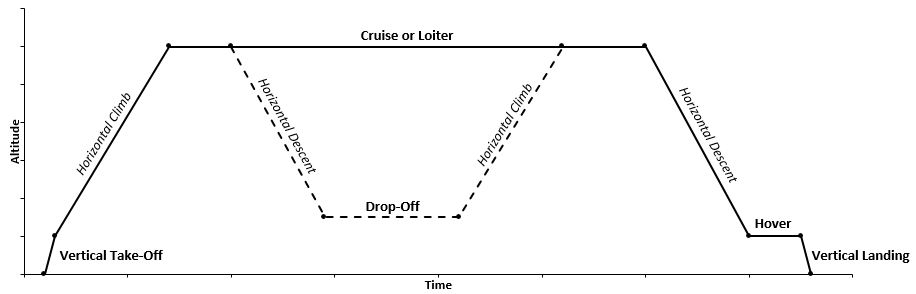
\includegraphics[scale=0.65]{ProjectDescription/Figures/Mission_Profile}
    \caption{Mission Profile for Different Missions}
    \label{fig:miss_prof}
\end{figure}

\section{Functional Analysis}
\label{ch:func_anal}
\setlength{\parindent}{15pt}

In this section the functions of the UAV are analysed by means of illustrating the functional flow diagram and functional breakdown structure. 

\subsection{Functional Flow Diagram}

The functional flow diagram is illustrated in \autoref{fig:FuncFlow}. The top-level flow of each mission is given on top of the figure. Each rectangle corresponds to a specific function to be performed and can be further elaborated on in a function-branch indicated by REF. Depending on the statement, a GO (G) or NO GO ($\overline{G}$) may follow the function. 

\begin{figure}[htb]
\centering
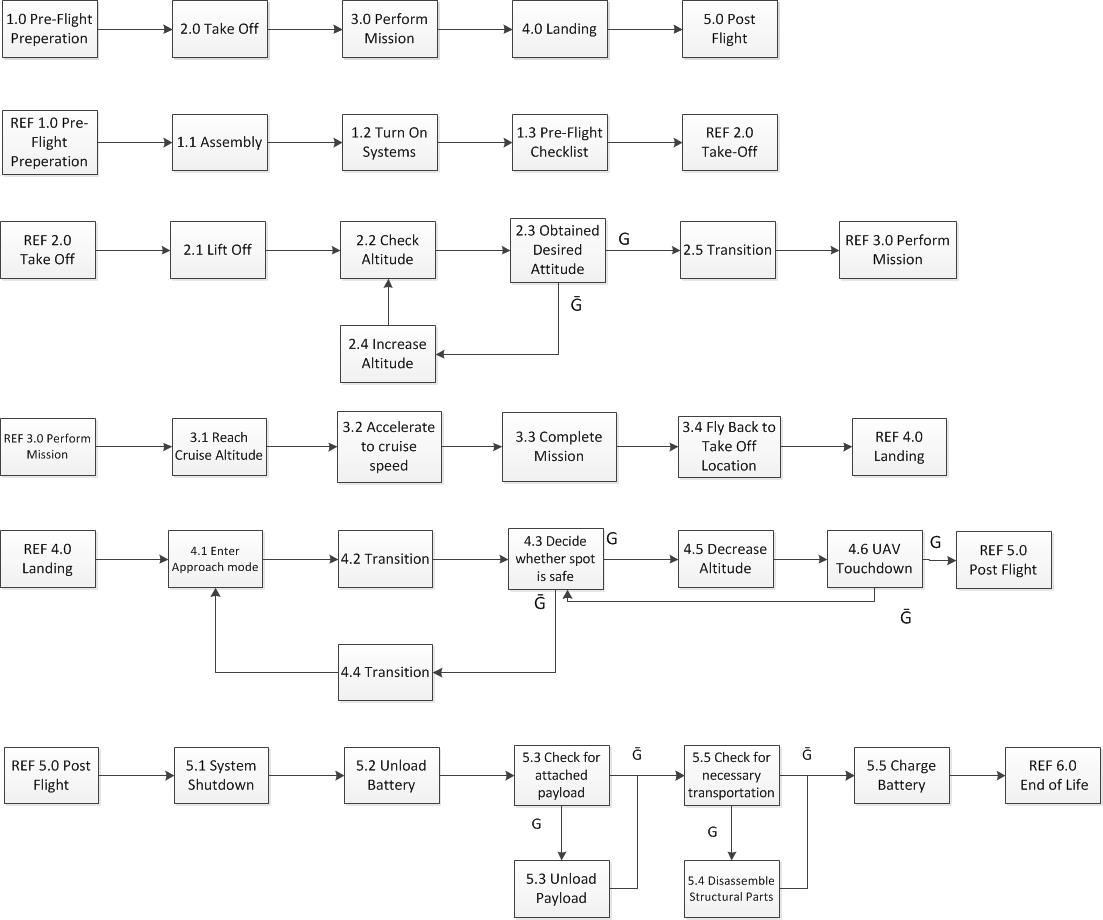
\includegraphics[width=\textwidth]{./ProjectDescription/Figures/ALL}
\caption{Functional Flow Diagram}
\label{fig:FuncFlow}
\end{figure}

The functional flow diagram is applicable to all missions stated in \autoref{sec:miss_desc}. First, the pre-flight preparations are carried out. Secondly, take-off and transition take place, after which the mission is performed. Finally, the transition and landing is carried out, followed by the post-flight procedures. Each mission phase consists of flying at cruise altitude and cruise speed towards the mission destination. However, function 3.3 Complete Mission is a mission specific function block. Depending on what mission the UAV has to fly, the UAV will have to perform different functions such as hovering, loitering, dropping of packages, etc.

\subsection{Functional Breakdown Structure}

\autoref{fig:FBS} shows the functional breakdown diagram where all top-level functions combined make the UAV system operative. The general structure was adapted from an example air transport mission \cite{SE_notes_2006}. The basic function of performing air transport is separated from performing missions and operates under various conditions. ``Perform air transport" breaks down the pre-flight operations, take-off preparations, flight operations and post-landing operation mission phases into functions. Since the flight operations are both important and extensive, they have a separate break-down in \autoref{fig:FBS-FlightOps}. 

It can be identified that the main missions are monitoring missions, transport missions between bases, transport mission with aerial drop-off, and combinations of them. Hence, functions must exist that enable those operations, e.g. the ability to follow predefined way points. The conditions under which these missions can be performed can be grouped into: normal operating conditions, under which the UAV can achieve its maximum performance, abnormal conditions, where limited flight operations are still possible, and emergency situations, in which safety considerations overrule the original mission. 


\begin{figure}[htb]
\centering
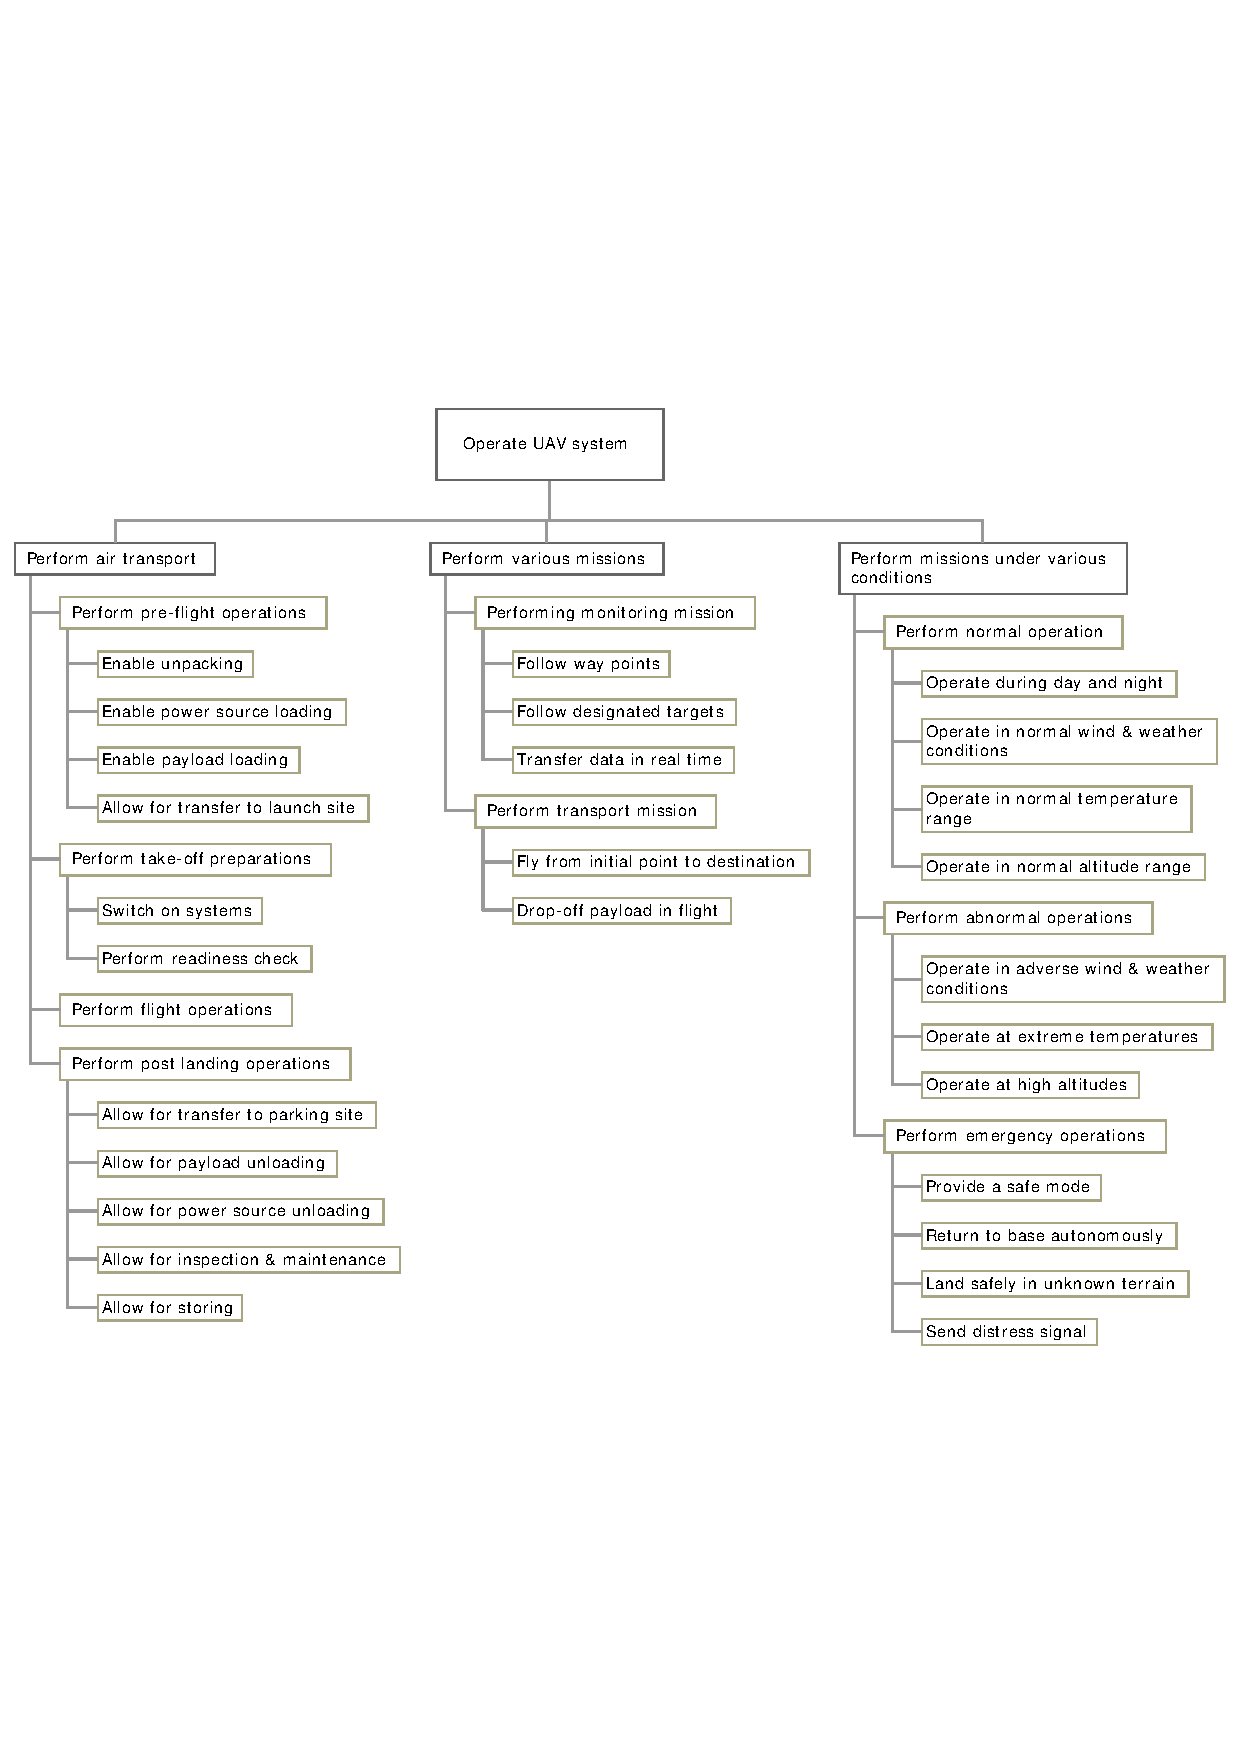
\includegraphics[width=\textwidth]{./ProjectDescription/Figures/FBS}
\caption{Functional Breakdown Structure}
\label{fig:FBS}
\end{figure}

\begin{figure}[htb]
\centering
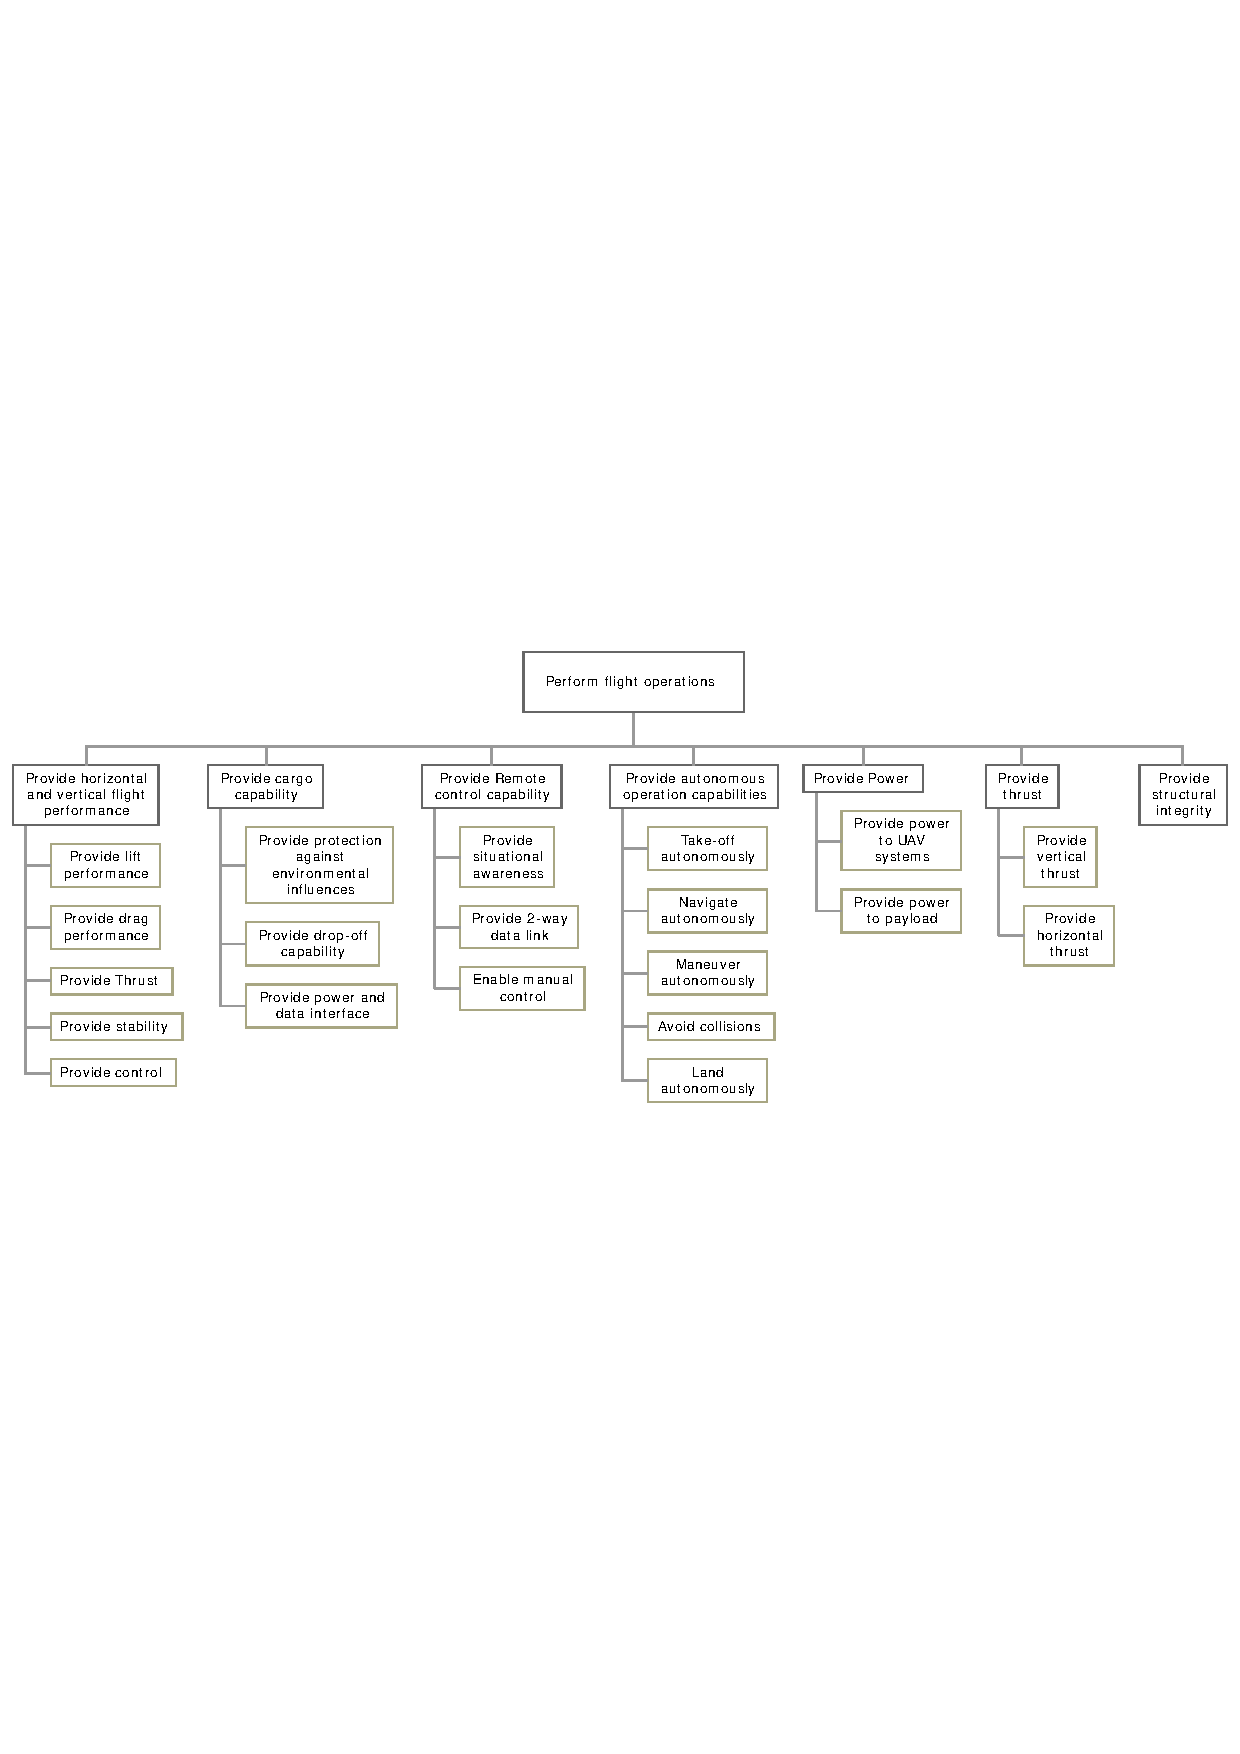
\includegraphics[width=\textwidth]{./ProjectDescription/Figures/FBS-FlightOps}
\caption{Perform Flight Operations Function}
\label{fig:FBS-FlightOps}
\end{figure}


